\section{Steganalysis}
\label{steganalysis}
Steganalysis is the study of detecting information hidden with steganography and if possible, recover that information.
Because of the nature of steganography, it is not always obvious if a file has hidden information or not.
Therefore steganalysis is often applied on a large set of files, which are suspected of containing hidden data.
There are many different techniques used in detection of hidden data, some of these techniques are described below.
%TODO: add more to intro

\subsection{Detection}
\label{Detection}
Most steganography algorithms are able to hide data without any notable visual impact on images.
It is therefore hard if not impossible to detect if something is hidden by simply looking at the image.

Detection of hidden data is therefore done with statistical tools like looking at histograms, modified DCT coefficients and signatures of different steganography algorithms.

\paragraph*{Colour Histogram}
A colour histogram is a representation of the distribution of colours in an image. 
This can be used to detect unusual distributions of colour, which may occur when using modifying the least significant bit or bits of each colour channel.

\begin{figure}
	\centering
	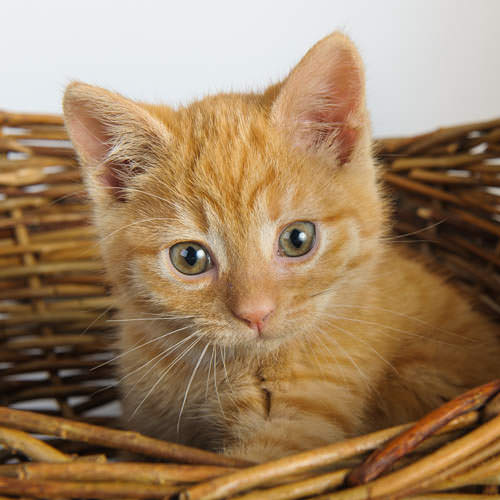
\includegraphics[width=0.4\textwidth]{figures/cover.jpg}
	\caption{Cover image.}
	\label{fig:CoverImage}
\end{figure}

\begin{figure}
	\centering
	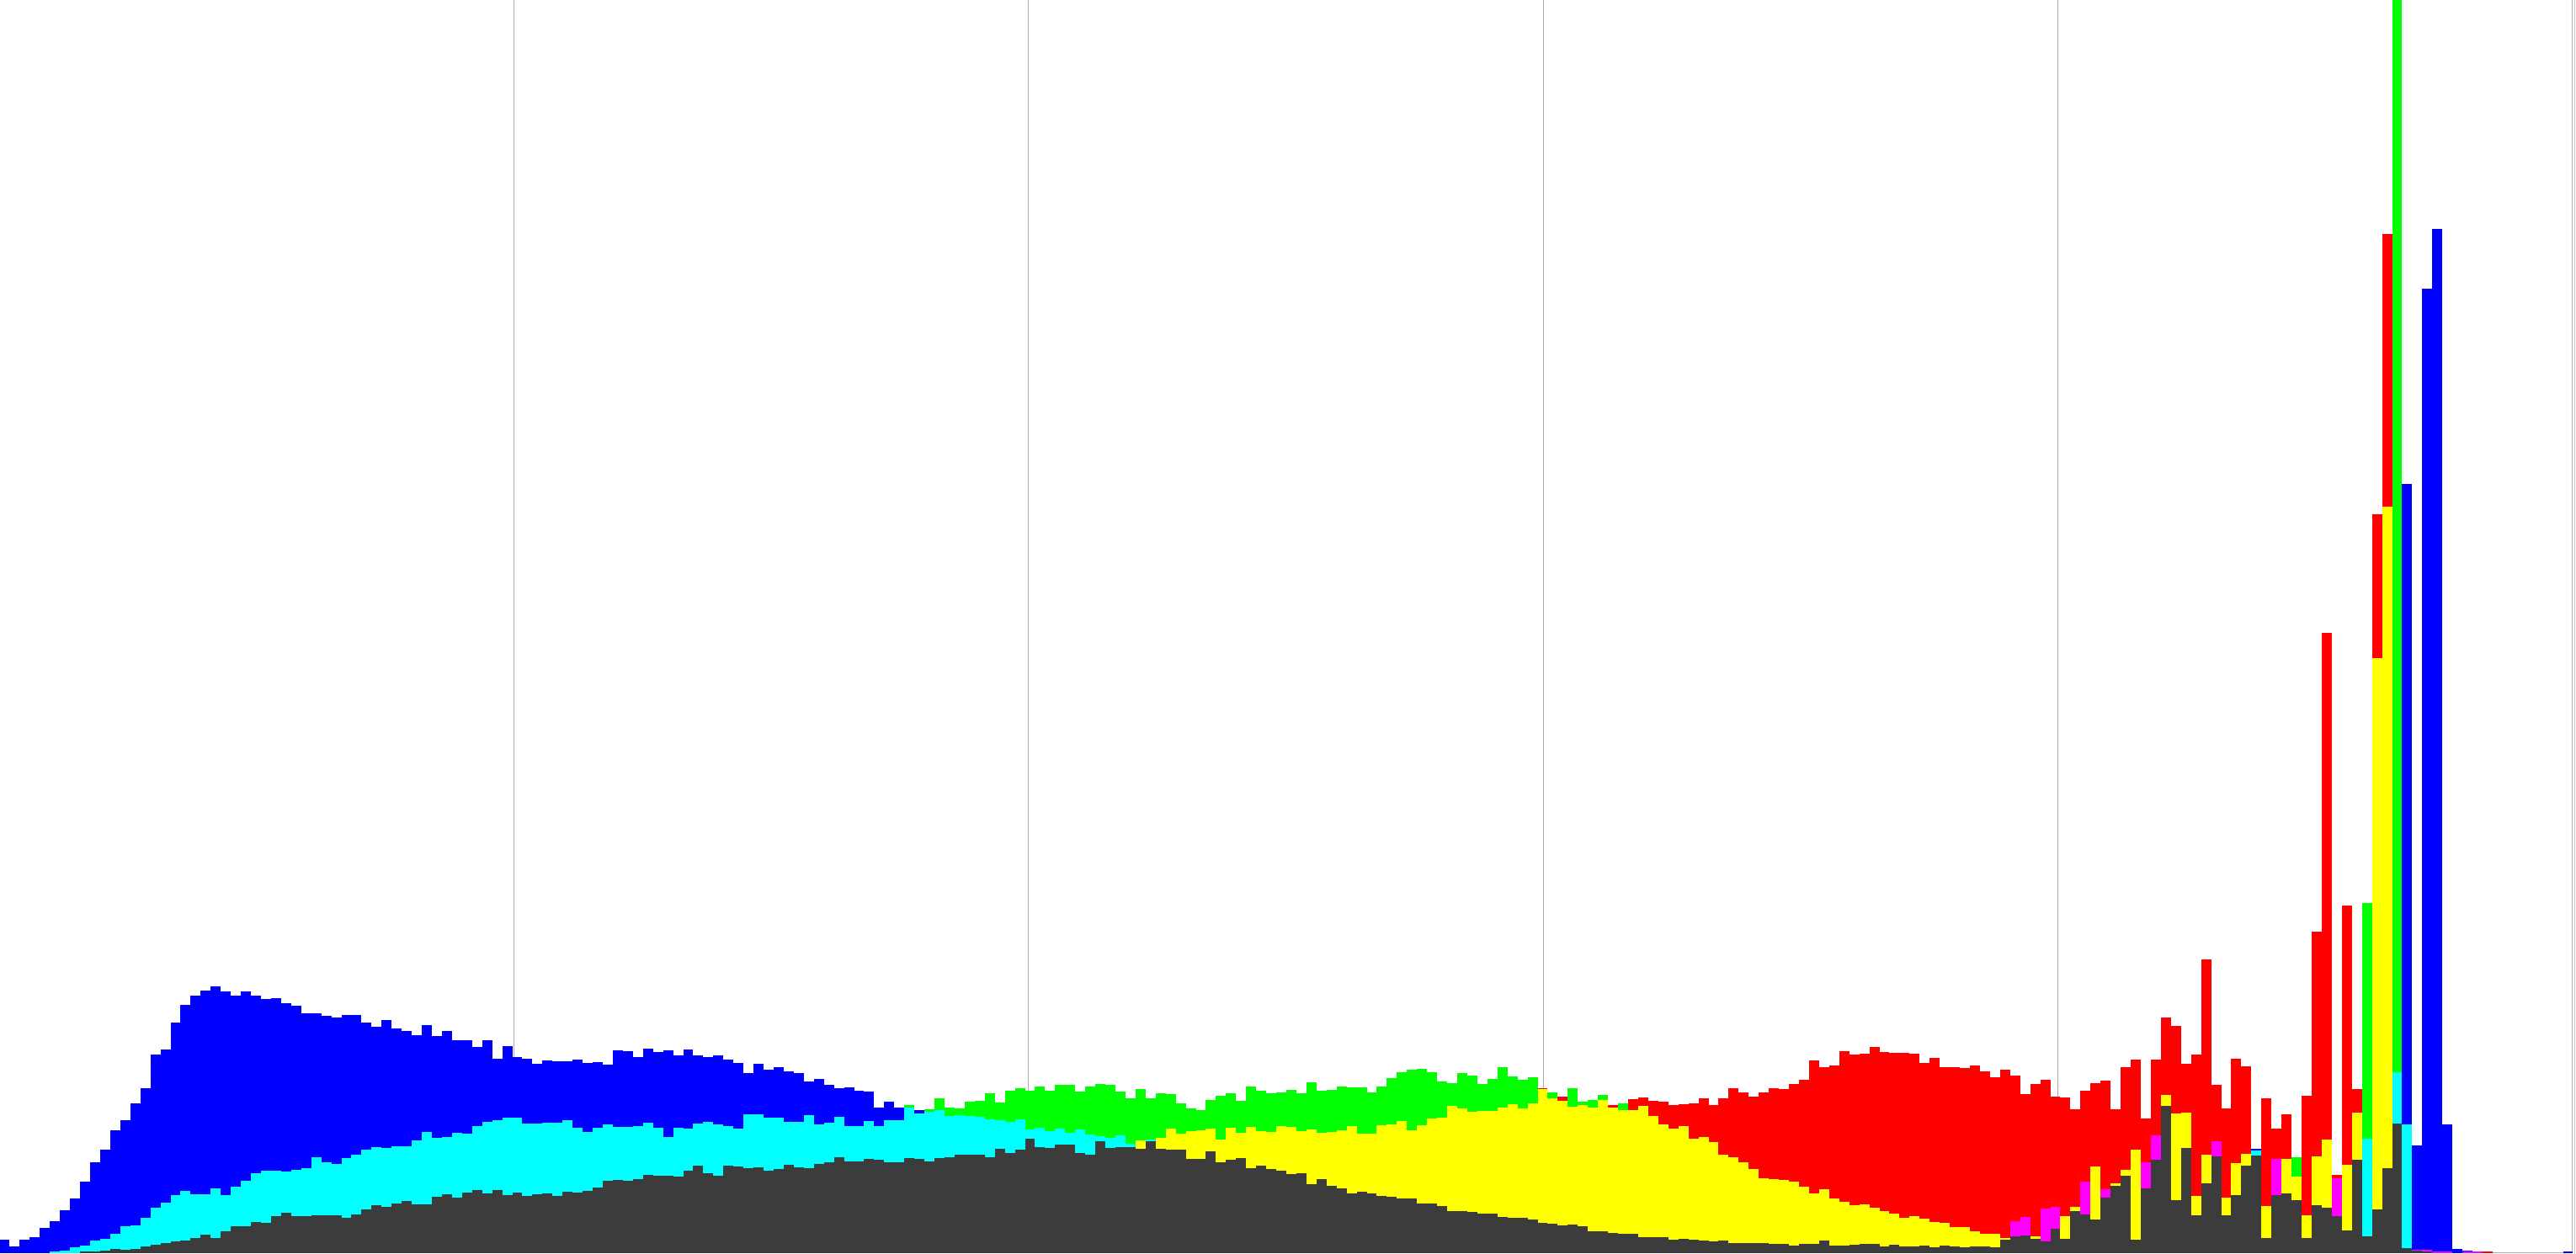
\includegraphics[width=0.6\textwidth]{figures/HistoLSBCat.png}
	\caption{Colour Histogram of image without hidden data.}
	\label{fig:HistoWithoutLSB}
\end{figure}

\begin{figure}
	\centering
	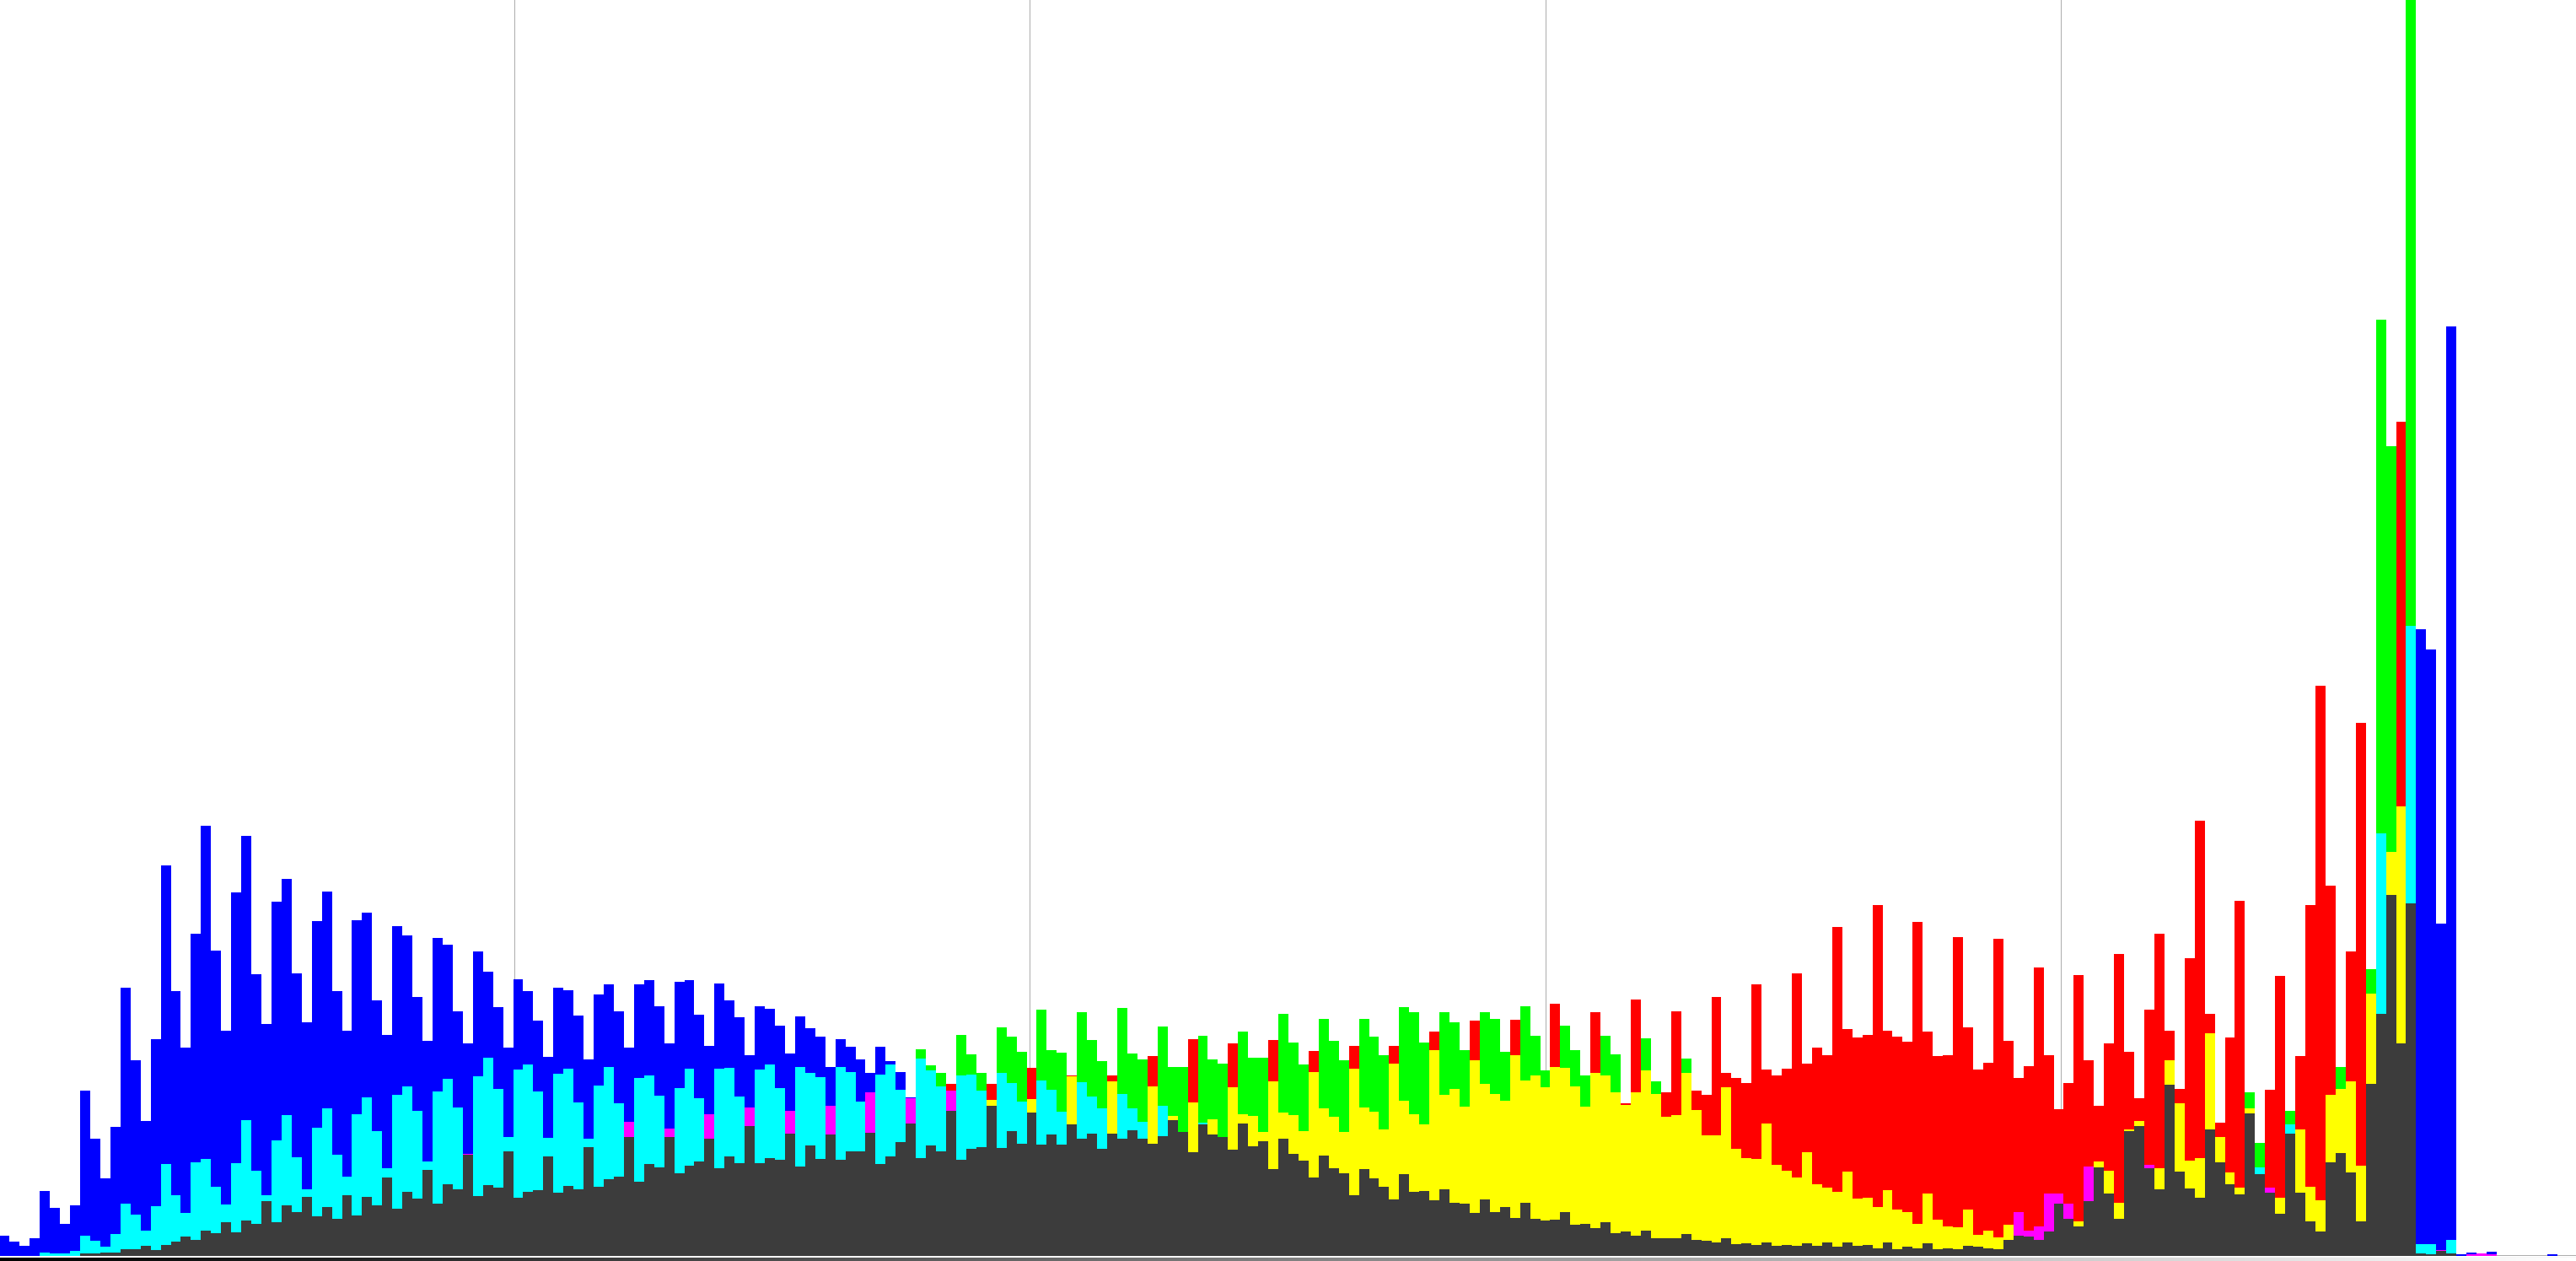
\includegraphics[width=0.6\textwidth]{figures/HistoLSBCatEncrypted.png}
	\caption{Colour Histogram of image containing secret image hidden with LSB.}
	\label{fig:HistoWithLSB}
\end{figure}

We have our cover image \ref{fig:CoverImage} and its respective colour histogram in figure \ref{fig:HistoWithoutLSB}.
We then hide another image in our cover image, this produces a new colour histogram (figure \ref{fig:HistoWithLSB}).
The new stego image has quite an unusual histogram, though sadly we cannot be sure there is hidden data only by looking at these histogram.

This unusual histogram might just be a product of a compression algorithm.

\paragraph*{DCT coefficients histogram}
By looking at a histogram of the DCT coefficients of a JPEG image, one might be able to detect if data has been hidden.
This is because of steganography algorithms like F5, the ``shrinkage'' it uses will result in a high amount of zeros in the DCT coefficients.
This can be seen on the comparison between figure \ref{fig:InputF5} and figure \ref{fig:outputF5}, these are histograms of DCT coefficients of figure \ref{fig:puffin}.
We can clearly see that after data has been hidden using the F5 algorithm there has occurred ``shrinkage'', with almost only zeros remaining.


\begin{figure}
	\centering
	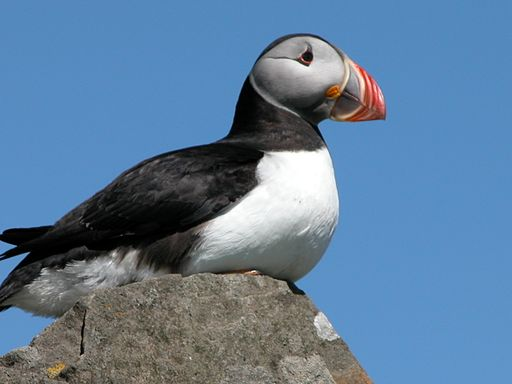
\includegraphics[width=0.25\textwidth]{figures/puffin.jpg}
	\caption{F5 cover image.}
	\label{fig:puffin}
\end{figure}

\begin{figure}
	\centering
	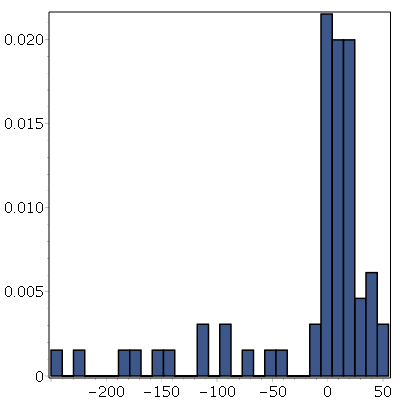
\includegraphics[width=0.5\textwidth]{figures/inputF5.png}
	\caption{Histogram of DCT coefficient before F5.}
	\label{fig:InputF5}
\end{figure}

\begin{figure}
	\centering
	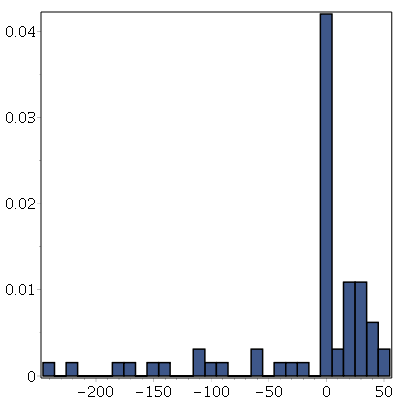
\includegraphics[width=0.5\textwidth]{figures/outputF5.png}
	\caption{Histogram of DCT coefficient after F5.}
	\label{fig:outputF5}
\end{figure}

%To estimate the DCT coefficients of the original cover image, we need to crop the suspected image by 4 vertical columns and recompress it using the same quantization table. \ref{Fridrich2003}
%TODO: add F5 to section "State of the art"

\paragraph*{LSB enhancing}
LSB enhancing works by doing the opposite of what LSB usually does, it eliminates all 7 high-level bits for each pixel except the last LSB. 
So all bytes will be either 0 or 1, it then ``enhances'' each byte by setting the 0 bytes to the minimum 0 and 1 to the maximum 255.
This make the LSB of the image very visible, allowing for a visual check by simply looking for patterns.
Figure \ref{fig:hiddengoodle} shows a 24 bit BMP image with 2 kb of random data hidden in it, and figure \ref{fig:LSBenhanced} is the same image LSB enhanced.
We can see that there is something hidden in the bottom half of the image, while the top half remains untouched\citep{Westfeld2000}.

\begin{figure}
	\centering
	
\includegraphics[width=0.4\textwidth]{figures/google.png}
	\caption{24 bit bmp image 2 kb random data.}
	\label{fig:hiddengoodle}
\end{figure}

\begin{figure}
	\centering
	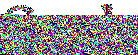
\includegraphics[width=0.4\textwidth]{figures/LSBenhanced.png}
	\caption{24 bit bmp image LSB enhanced.}
	\label{fig:LSBenhanced}
\end{figure}

%\paragraph*{$\chi^2$ attack or chi-squared attack}
%Chi-squared is a statistical test measure if a given set observed data and an expected set of data are similar.
%We compare pairs of values' observed frequencies with their expected frequencies and calculate the probability of having some embedded data.
%\ref{fig:Chiattack} shows the result of chi-squared attack on figure \ref{fig:hiddengoodle}.

\paragraph*{Steganography signatures}
Unusual patterns in a image are obvious and arise suspicion, for example unused bits in the file headers or even comment headers, these might give us some insight into which algorithm was used.

\subsection{Recovery}
Recovery of data hidden with steganography is difficult, to recover the data we must know what kind of algorithm was used to hide the data.
Even if we know the algorithm used, we might still only get back meaningless data, because in addition to hiding the data, it might also be encrypted.

So the most common way of recovering hidden data is by using the same algorithm that was used to encode the image to decode the data.
%\begin{figure}
%	\centering
%	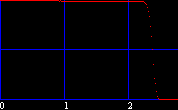
\includegraphics[width=0.5\textwidth]{figures/ChiSquareAttack.png}
%	\caption{Graph of chi-squared attack.}
%	\label{fig:Chiattack}
%\end{figure}
